\subsection{Phân tích lỗi ghép cặp và theo lớp}
\label{sec:errors}
\subsubsection{Định nghĩa được giúp và bị làm sai}
Với cùng mã ảnh, mức suy giảm, noise seed và checkpoint, gọi $b_i,e_i,y_i$ là dự đoán Identity, dự đoán sau xử lý và nhãn thật:
\begin{align}
H&=\sum_i\mathbf1[b_i\ne y_i,\ e_i=y_i],\\
D&=\sum_i\mathbf1[b_i=y_i,\ e_i\ne y_i].
\end{align}
Với $N$ ảnh ghép cặp, $\Delta\mathrm{Accuracy}=100(H-D)/N$ điểm phần trăm. Quan hệ này kiểm tra tính nhất quán; không dùng $H-D$ thay cho thay đổi Macro-F1. Hai nhóm còn lại là cùng đúng và cùng sai; nhóm cùng sai vẫn có thể đổi sang lớp sai khác.
\par
\begin{table}[!htbp]\centering
\caption{Số ảnh trung bình được giúp ($H$), bị làm sai ($D$) mỗi lượt full-test 12.630 ảnh. Trung bình qua noise seed và checkpoint, không phải ảnh nguồn độc lập.}
{\small\begin{tabular}{llrrr}\toprule Phương pháp & Mức & $H$ & $D$ & $\Delta$ Acc. (đpt)\\\midrule
\tableinput{tables/paired_transitions}\bottomrule\end{tabular}}\label{tab:transitions}\end{table}\par


Ở mức vừa, Gaussian rồi Gamma sửa đúng trung bình 1472,67 ảnh nhưng làm sai 29,22 ảnh mỗi lượt, tăng ròng 1443,44 ảnh, tương ứng 11,43 điểm phần trăm Accuracy. Lợi ích tổng thể vẫn đi kèm nhóm mẫu bị ảnh hưởng bất lợi. Tính cả hai hướng chuyển giúp tránh chỉ trình bày ví dụ được cải thiện.

\clearpage
\subsubsection{Ma trận nhầm lẫn và các cặp nhầm}
Ma trận $C_{ab}$ có hàng là nhãn thật và cột là dự đoán. Chuẩn hóa hàng bằng support lớp thật giúp xem recall và cặp nhầm dù full-test mất cân bằng lớp.
\fig{confusions_detail_1.png}{0.82}{Ma trận chuẩn hóa hàng của Identity và CLAHE, full-test mức nặng, checkpoint 11, noise seed 101. Mỗi hàng là một lớp thật; cột 5 biểu thị dự đoán giới hạn 80 km/h.}{fig:confusions}
\clearpage
\fig{confusions_detail_2.png}{0.82}{Ma trận của diffusion và Gaussian rồi Gamma trên cùng 12.630 ảnh, mức, checkpoint và noise seed như Hình~\ref{fig:confusions}. Đây là một lát cắt xác định, không phải ma trận trung bình qua seed.}{fig:confusionsdetail}
\clearpage
\par
\begin{table}[!htbp]\centering
\caption{Ba cặp nhầm có tỷ lệ trung bình cao nhất của mỗi phương pháp ở mức nặng, full-test. Mẫu nguồn dùng chung giữa các lượt.}
{\small\begin{tabular}{lrrr}\toprule Phương pháp & Lớp thật & Lớp dự đoán & Tỷ lệ (\%)\\\midrule
\tableinput{tables/confusion_pairs}\bottomrule\end{tabular}}\label{tab:pairs}\end{table}\par

\subsubsection{Hiện tượng tập trung dự đoán vào lớp 5}
Lớp 5 là biển giới hạn 80 km/h, có 630/12.630 ảnh, tương ứng 4,99\% full-test. Định nghĩa $q_5=\sum_a C_{a5}/N$ là tỷ lệ dự đoán lớp 5 và $e_5=(\sum_a C_{a5}-C_{55})/N$ là tỷ lệ toàn bộ ảnh bị gán sai vào lớp này. Precision lớp 5 đo phần dự đoán 80 km/h thực sự đúng. Mỗi chỉ số được tính riêng từng lượt rồi tổng hợp theo noise seed và checkpoint.

\par\begin{table}[!htbp]\centering
\caption{Tập trung dự đoán vào lớp 5 ở mức nặng, đơn vị \%. Hai cột đầu lấy mẫu số là toàn bộ 12.630 ảnh/lượt; precision dùng số ảnh được dự đoán lớp 5.}
{\small\begin{tabular}{lrrr}\toprule Phương pháp & Dự đoán lớp 5 & Gán sai vào lớp 5 & Precision lớp 5\\\midrule
\tableinput{tables/class5_concentration}\bottomrule\end{tabular}}\label{tab:classfive}
\end{table}\par

Identity dự đoán lớp 5 cho 43,17\% ảnh dù tỷ lệ thật chỉ là 4,99\%; 38,32\% toàn tập bị gán sai vào lớp này. Gaussian rồi Gamma giảm tỷ lệ dự đoán lớp 5 còn 28,97\% nhưng vẫn tập trung mạnh; precision lớp 5 chỉ đạt 17,16\%. Diffusion có tỷ lệ dự đoán lớp 5 thấp hơn, 8,99\%, dù Macro-F1 tổng thể thấp hơn chuỗi được chọn. Như vậy, ưu thế trung bình không đồng nghĩa mọi kiểu lỗi đều được giảm tốt nhất.

Các cột 5 đậm và những cặp nhầm như lớp 10/6/30 sang lớp 5 phản ánh xu hướng dồn quyết định về một lớp khi suy giảm nặng. Mất tương phản, nét số nhỏ và sai khác miền đầu vào là các giả thuyết phù hợp để kiểm tra; ma trận chưa chứng minh nguyên nhân nằm riêng ở màu hay hình dạng. Chưa đo activation, độ nhạy theo vùng hoặc so phân bố train nên không quy hiện tượng này trực tiếp cho mất cân bằng lớp. Sáu ảnh kiểm chứng ở phần sau cho thấy cả sửa đúng lẫn phát sinh nhầm 60 thành 80 km/h.


\subsubsection{Các lớp khó và ví dụ có metadata}
\fig{per_class_severe_detail.png}{1}{F1 từng lớp mức nặng trên full-test, tách lớp 0--21 và 22--42 để dễ đọc. Trung bình noise trong checkpoint rồi trung bình ba checkpoint; không phải khoảng tin cậy của camera thực.}{fig:classf1}
\par
\begin{table}[!htbp]\centering
\caption{Năm lớp có F1 thấp nhất của Gaussian rồi Gamma mức nặng. SD qua checkpoint sau trung bình noise; chênh lệch so Identity là điểm phần trăm.}
\begin{tabular}{rrrr}\toprule Class ID & F1 (\%) & SD & $\Delta$ F1\\\midrule
\tableinput{tables/hard_classes}\bottomrule\end{tabular}\label{tab:hardclasses}\end{table}\par


Macro-F1 tăng không có nghĩa mọi lớp đạt hiệu năng tốt. Các lớp khó vẫn có F1 thấp và cần xem cùng support, cặp nhầm và ảnh nguồn. Không quy một cặp nhầm chắc chắn cho mất nét số hoặc sai màu chỉ từ ma trận; đó là giả thuyết cần quan sát ảnh cụ thể để xác nhận.
\clearpage
\subsubsection{Đối chiếu trực quan sáu mẫu kiểm chứng}
Hình~\ref{fig:visualcases} dùng full-test mức vừa, checkpoint 11 và noise seed 101; mỗi nhóm lấy hai ID nhỏ nhất. Ảnh được cắt lại từ PPM chính thức theo đúng ROI, lề và phép nội suy; cả 12 dự đoán trên ảnh tối và ảnh xử lý đều khớp CSV đã kiểm chứng. Nhãn sáu ảnh được đối chiếu với annotations chính thức.

\begin{center}
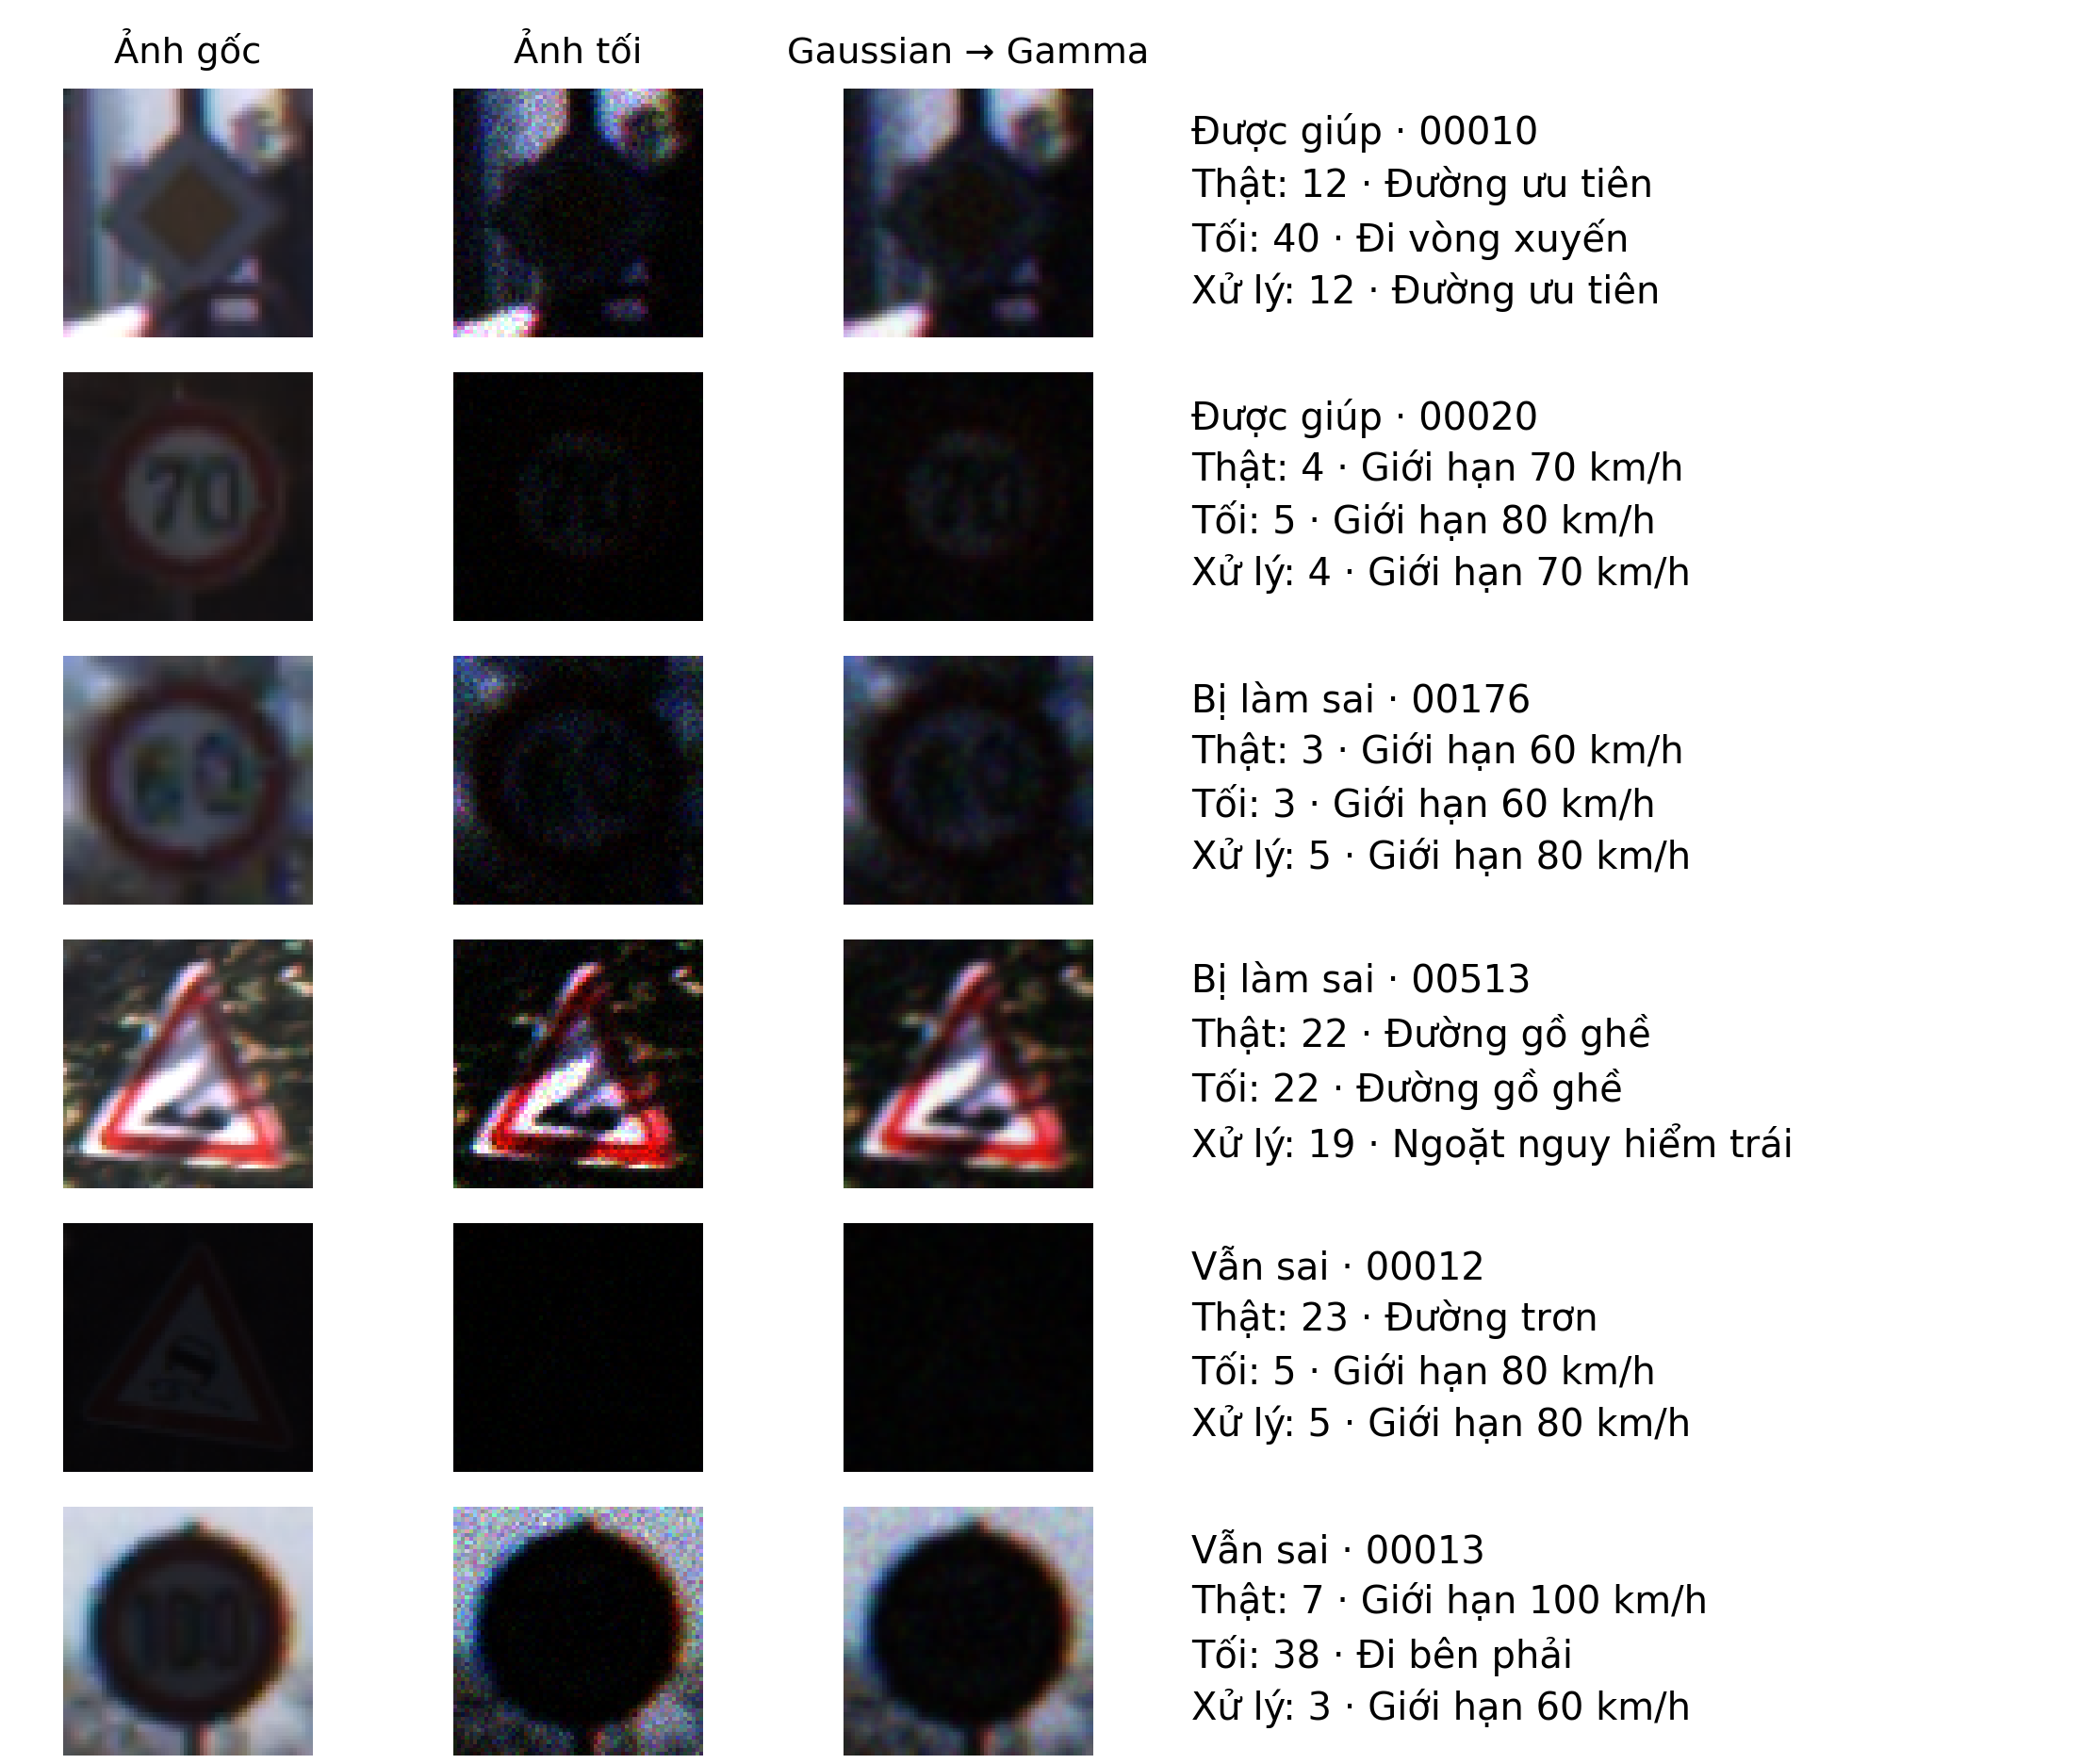
\includegraphics[width=\linewidth]{visual_error_cases.png}
\captionof{figure}{Ảnh gốc, ảnh tối và Gaussian rồi Gamma trên cùng sáu mẫu GTSRB~\cite{gtsrbdata}. Tên biển đi kèm Class ID; ID ảnh là phần cuối của \texttt{gtsrb/test/<ID>}. Các ảnh dùng cùng thang RGB, phóng bằng láng giềng gần nhất, không tự cân bằng sáng để hiển thị.}
\label{fig:visualcases}
\end{center}

{\fontsize{11bp}{13bp}\selectfont
\textbf{Được giúp:} 00010 đổi từ vòng xuyến sang đúng đường ưu tiên; 00020 đổi từ giới hạn 80 sang đúng 70 km/h. Nhiễu hạt giảm sau lọc, nhưng đầu ra vẫn tối; nhận dạng đúng không đòi hỏi ảnh phải sáng rõ hoàn toàn.\par
\textbf{Bị làm sai:} 00176 đổi từ đúng 60 sang 80 km/h; 00513 đổi từ đúng đường gồ ghề sang ngoặt trái. Ảnh xử lý ít hạt hơn nhưng nét nhỏ vẫn mềm; giảm nhiễu không bảo đảm giữ đặc trưng phân lớp.\par
\textbf{Vẫn sai:} 00012 và 00013 còn rất tối sau xử lý, nét biểu tượng và chữ số chưa rõ đủ để dự đoán đúng. Hình cho phép quan sát hiện tượng, chưa xác định pixel hoặc cơ chế nào gây ra quyết định của CNN. Sáu mẫu không thay thế thống kê toàn tập.\par}
\clearpage
